\FloatBarrier
\subsection{Optical layout}\label{sec:optlayout}
%\emph{Author(s): \textbf{S.\ Hild}, A.\ Thuering, A.\ Freise \\}

This section describes the details of the ET optical layout, such 
as the laser beam sizes, beam shapes and distances between
optical components inside the arm cavities and central interferometer
including the power and signal recycling cavities. A schematic sketch
of
the optical layout of all core optical of the interferometers is shown
in figure~\ref{Fig:Simple_ETv1}.
Constraints imposed
onto the optical layout are briefly discussed in section~\ref{sec:opt_layout_class}, while 
section~\ref{sec:xylophone} lays out the motivation for choosing a dual-tone xylophone detector.
The optical layout of the arm cavities is discussed in detail in section~\ref{sec:arm_cavity_design}.
%and the corresponding effects of parametric instabilities are analysed in section~\ref{sec:opt_layout_PI}.
Finally section~\ref{sec:opt_layout_CITF} describes the layout of the recycling cavities. 

\begin{figure}[p]
\centering
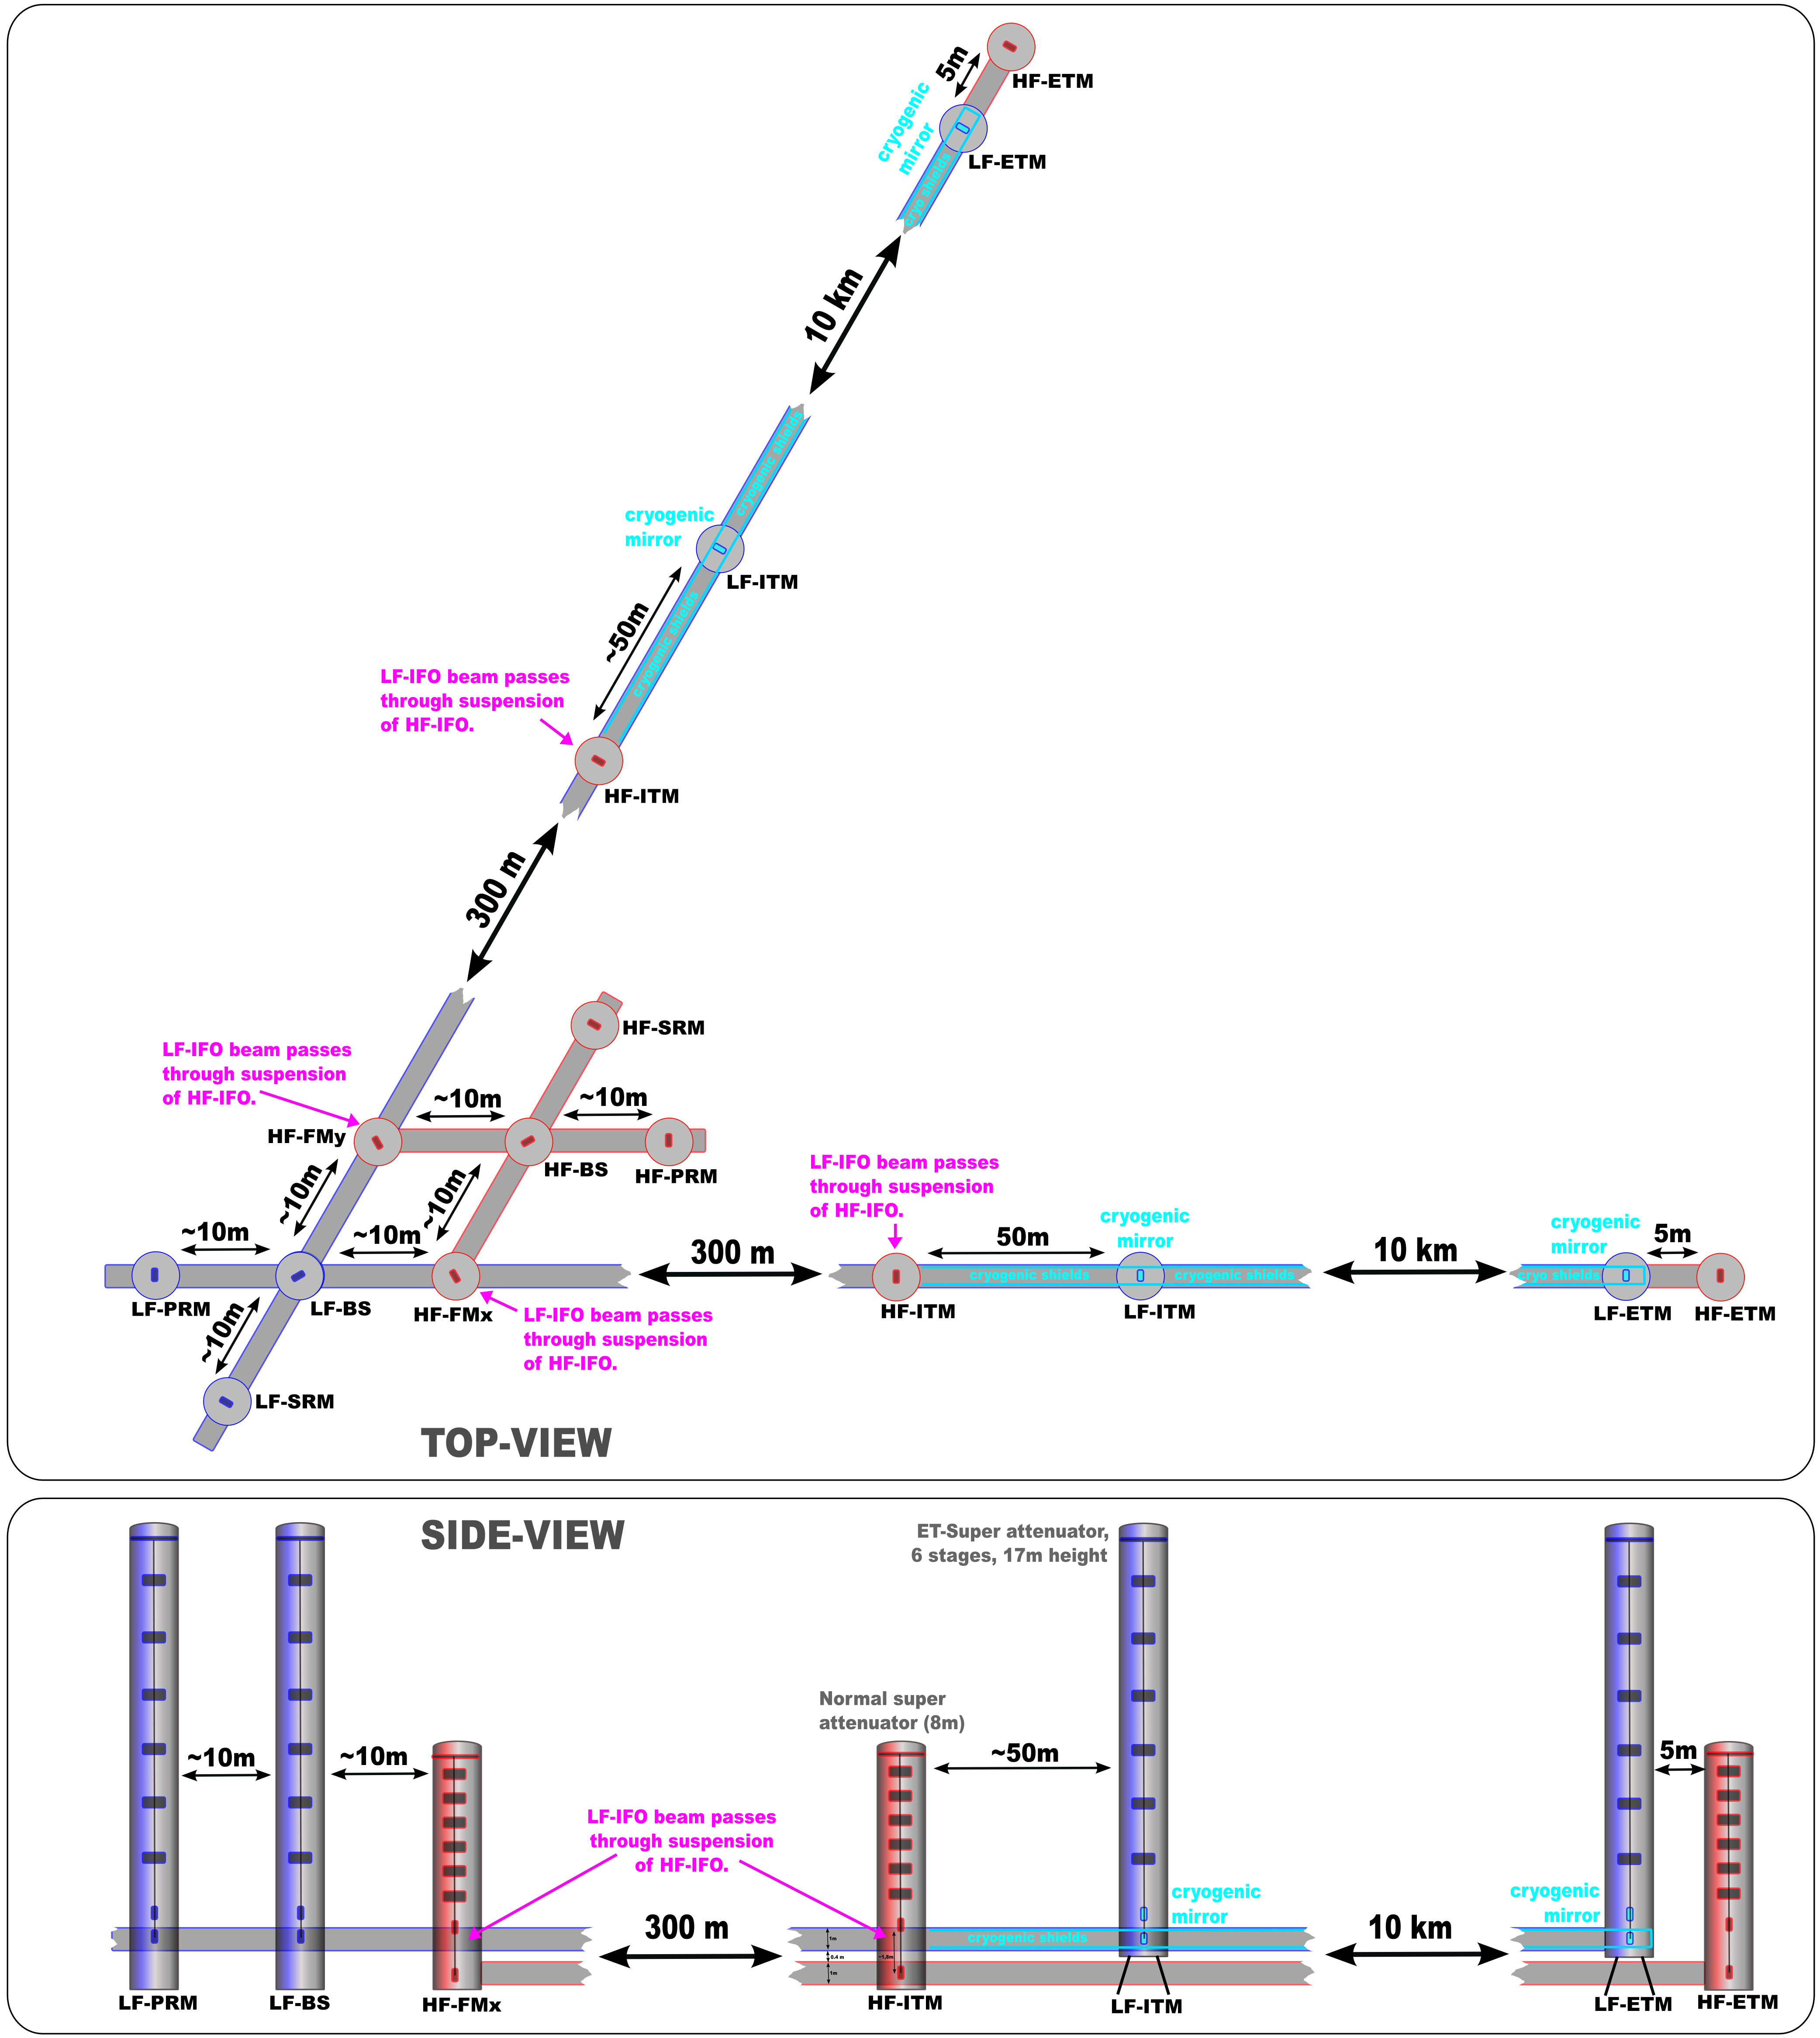
\includegraphics[width=1\textwidth]{Sec_Optics/ET_April2011_v2.png}
\caption{Simplified drawing of the low and high frequency core interferometers of a single ET-detector. Injection and
detection optics as well as filter cavities have been omitted for clarity. Please not that the complete ET observatory
consists of three such detectors.%
}
\label{Fig:Simple_ETv1}
\end{figure}


\subsubsection{Constraints on the optical layout from classical noise sources }
\label{sec:opt_layout_class}

Apart from the quantum noise there are many other noise sources,
usually called classical or technical noise sources, degenerating
the sensitivity of a laser interferometric gravitational-wave
detector. In the third generation of detectors these classical
noise sources have to be addressed with different techniques which
impose additional constraints onto the optical layout of the ET
interferometers.

The suspension thermal noise of the low frequency interferometers will
be one of the limiting noise sources at the low-frequency end of the 
ET detection band (for more details refer to Sec. \ref{sec:thermal_noise}).
In order to guarantee optimal
thermal noise performance, the fibers of the suspended optics---especially
those in a cryogenic environment---have to be be kept at 
their designed operating temperature. Since each detector consists of two
interferometers,  the question arises how to arrange the collinear
interferometer arms in the tunnel. One of the
interferometer arm could be placed above the other. In that case it is
 unavoidable that the laser beam of the interferometer on top
 intersects at some point with the suspension fibers
of the other interferometer. Therefore, we chose to arrange the individual 
interferometer beams in a way that the beams of the low-frequency interferometers
sit on top of the beams of the high-frequency interferometers. This configuration
ensures, that no high power laser beams comes close to any cryogenic 
suspension fibres and only the low power beams of the low frequency interferometers 
have to pass the between the rather uncritical fibres of the room temperature
 suspensions of the high frequency interferometers (see Figure \ref{Fig:Simple_ETv1}). 

%{\bf Mirror internal thermal noise.} \emph{Author(s): Keiko
%Kokeyama, Andreas Freise} 
The noise coming from thermal effects
influencing the test-mass mirrors is dominating the noise spectrum
in the mid frequency regime. There exist several different
contributions to the total thermal noise of which the coating
Brownian thermal noise is the largest in current interferometer
topologies utilizing arm cavities. The obvious way of lowering
the thermal noise contributions is cooling the mirrors down to cryogenic
temperatures. However, such cryogenic test-masses allow only for a  limited
amount of optical power passed through the mirror substrates and
coatings, which is the reason why we consider cryogenic mirrors
only for the low frequency interferometers.

 Another branch of techniques 
to lower the thermal noise is to increase the beam size on the test masses and change the mode of the
laser beam inside the interferometer (cf.\ Sec.~\ref{sec:thermalnoiseLG}).
The maximal practical beam sizes for the ET interferometers is given by
the the maximal available substrate
size on one hand  and the required cavity stability  one the other hand (see Sec \ref{sec:arm_cavity_design}). 
In order to obtain an optimal noise performance of the high-frequency interferometers we consider them 
to operate with laser beams of the Laguerre-Gauss (3,3)-mode (LG$_{33}$)~\cite{Mours06, Vinet2007}.
The limitation in using LG modes\footnote{All throughout this document, we refer to the so-called `helical' Laguerre-Gauss modes, whose intensity pattern is circularly symmetric. See e.g.\ definition in~\cite{Mours06}.} is that they can resonate only in cavities with an even number of mirrors. Therefore, no triangular cavity may be used.


\longetbox{i}{ibox:lg33}{The Laguerre Gauss LG$_{33}$ mode}{%
To reach the envisaged sensitivity for ET, the
thermal noise has to be reduced significantly with respect to Advanced detectors. So
far, no single technique or technology can achieve this but a
combination of methods needs to be employed. The current
design includes the use of the higher-order
Laguerre Gauss mode LG$_{33}$ instead of the 
standard, fundamental Gaussian TEM$_{00}$ beam for the high-power, high-frequency
interferometer. Laguerre-Gauss modes are commonly given
in their orthonormal form, see for example \cite{Living:Freise}:
\begin{equation}
\label{eq:uld1}
\begin{array}{rcl}
u_{p,l}(r,\phi,z)&=& \frac{1}{w(z)}\sqrt{\frac{2p!}{\pi(|l|+p)!}}\exp(\mathrm{i}\,(2p+|l|+1)\theta(z))\\
&\times&\left(\frac{\sqrt{2}r}{w(z)}\right)^{|l|}L_p^{(|l|)}\left(\frac{2r^2}{w(z)^2}\right) \exp\left(-\mathrm{i}\,
k\frac{r^2}{2q(z)}+\mathrm{i}\, l \phi\right),
\end{array}
\end{equation}
with $r$, $\phi$ and $z$ as the cylindrical coordinates around the
optical axis. The letter $p$ is the radial mode index, $l$ the
azimuthal mode index and $L_p^{(l)}(x)$ are the associated
Laguerre polynomials.
%
%\begin{equation}
%L_p^{(l)}(x)=\frac{1}{p!}\sum_{j=0}^p\frac{p!}{j!}
%\left(
%\begin{array}{c}
%l+p\\
%p-j
%\end{array}\right)(-x)^j .
%\end{equation}
%
The other parameters used in equation~\ref{eq:uld1} are defined as
follows:
$w_0$ is the beam radius at the \emph{beam waist} and $z_0$ the
position of the beam waist along the $z$-axis. %$z_{\mathrm{R}}$ is the
                                %Rayleigh range, 
$w$ is the beam radius,
$q$ is called the \emph{Gaussian beam
  parameter} and
$\theta$ is the Gouy phase.
%%%%%%%%%%%
The LG$_{33}$ 
is shown in Fig.~\ref{Fig:LG33}, it provides wider intensity pattern
which directly reduces the impact of thermal noise as well as
thermal lensing. The spherical phase front makes it possible to use
this mode with spherical mirrors.
\begin{figure}[H]
\centering
     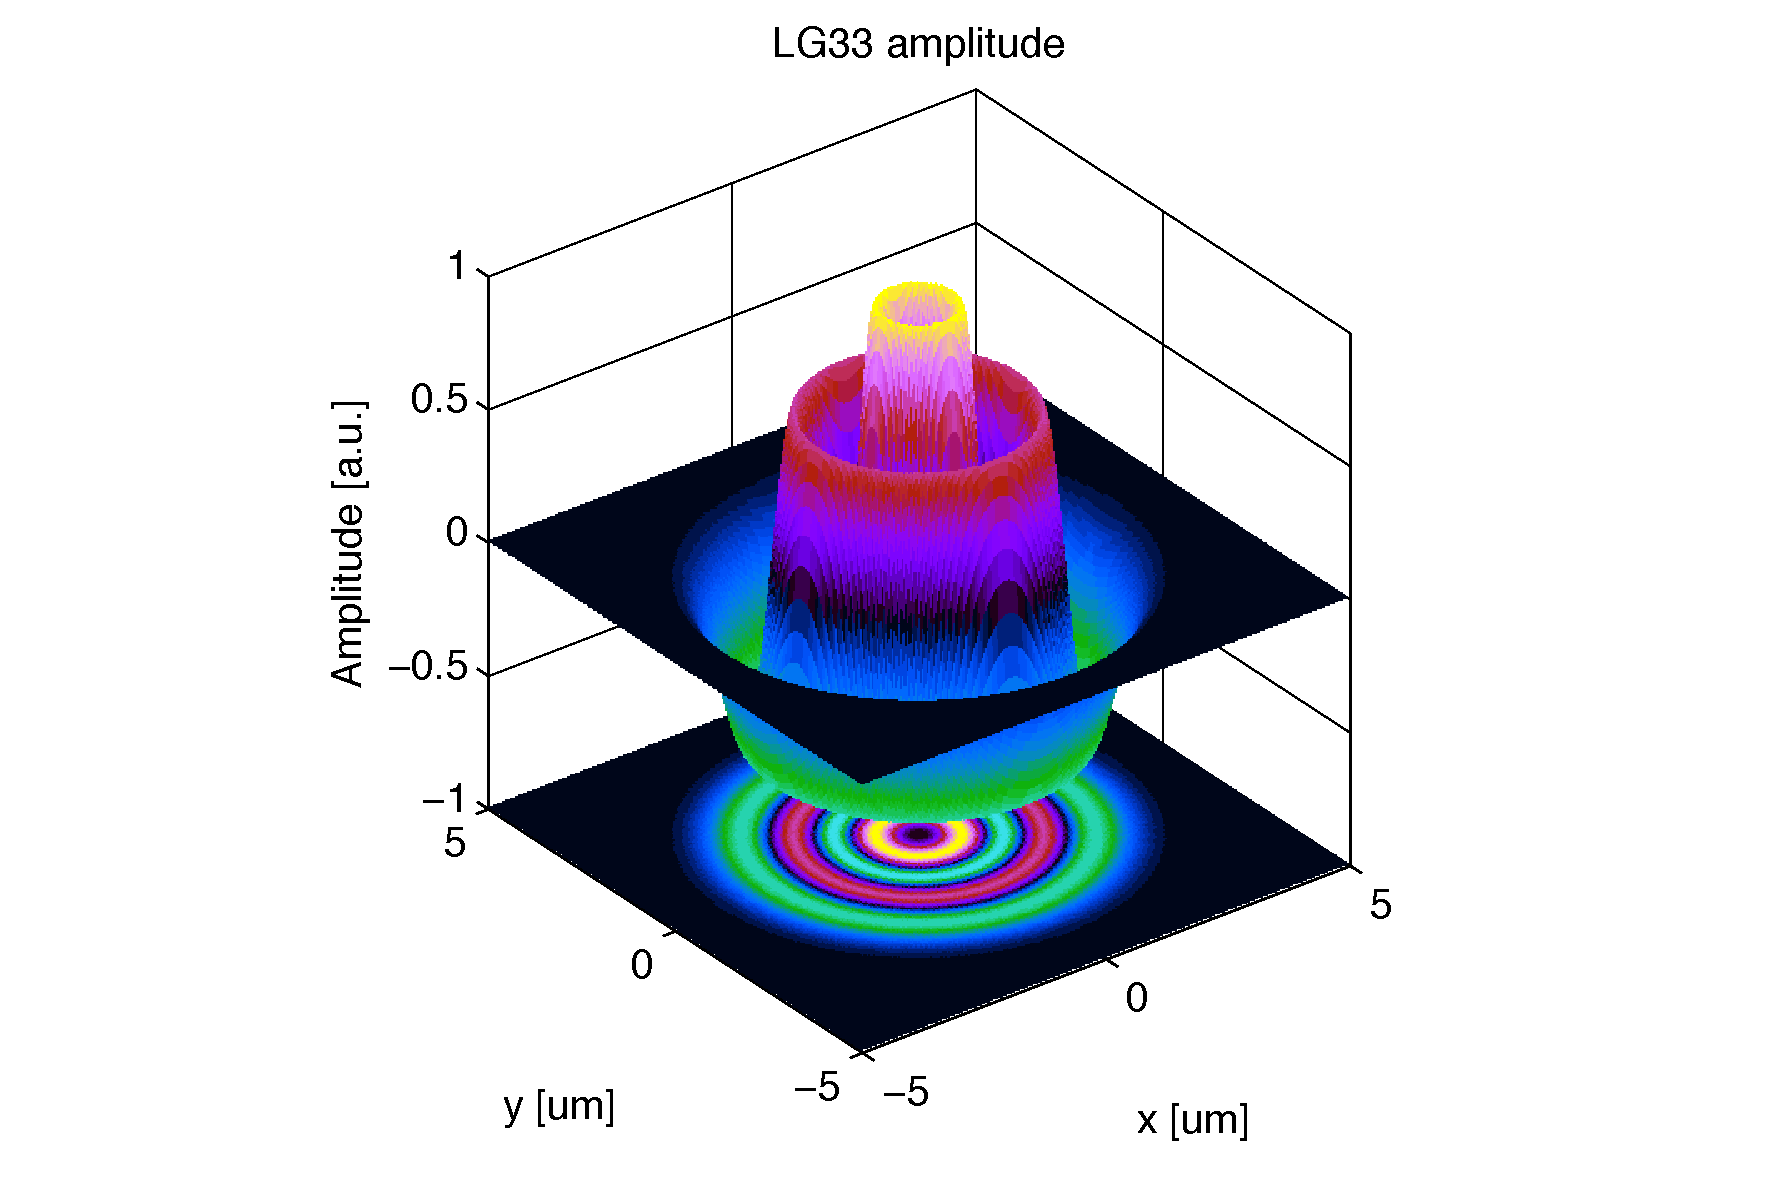
\includegraphics[width=0.47\textwidth, viewport=180 0 740 530]{Sec_Optics/LG33_amp}
      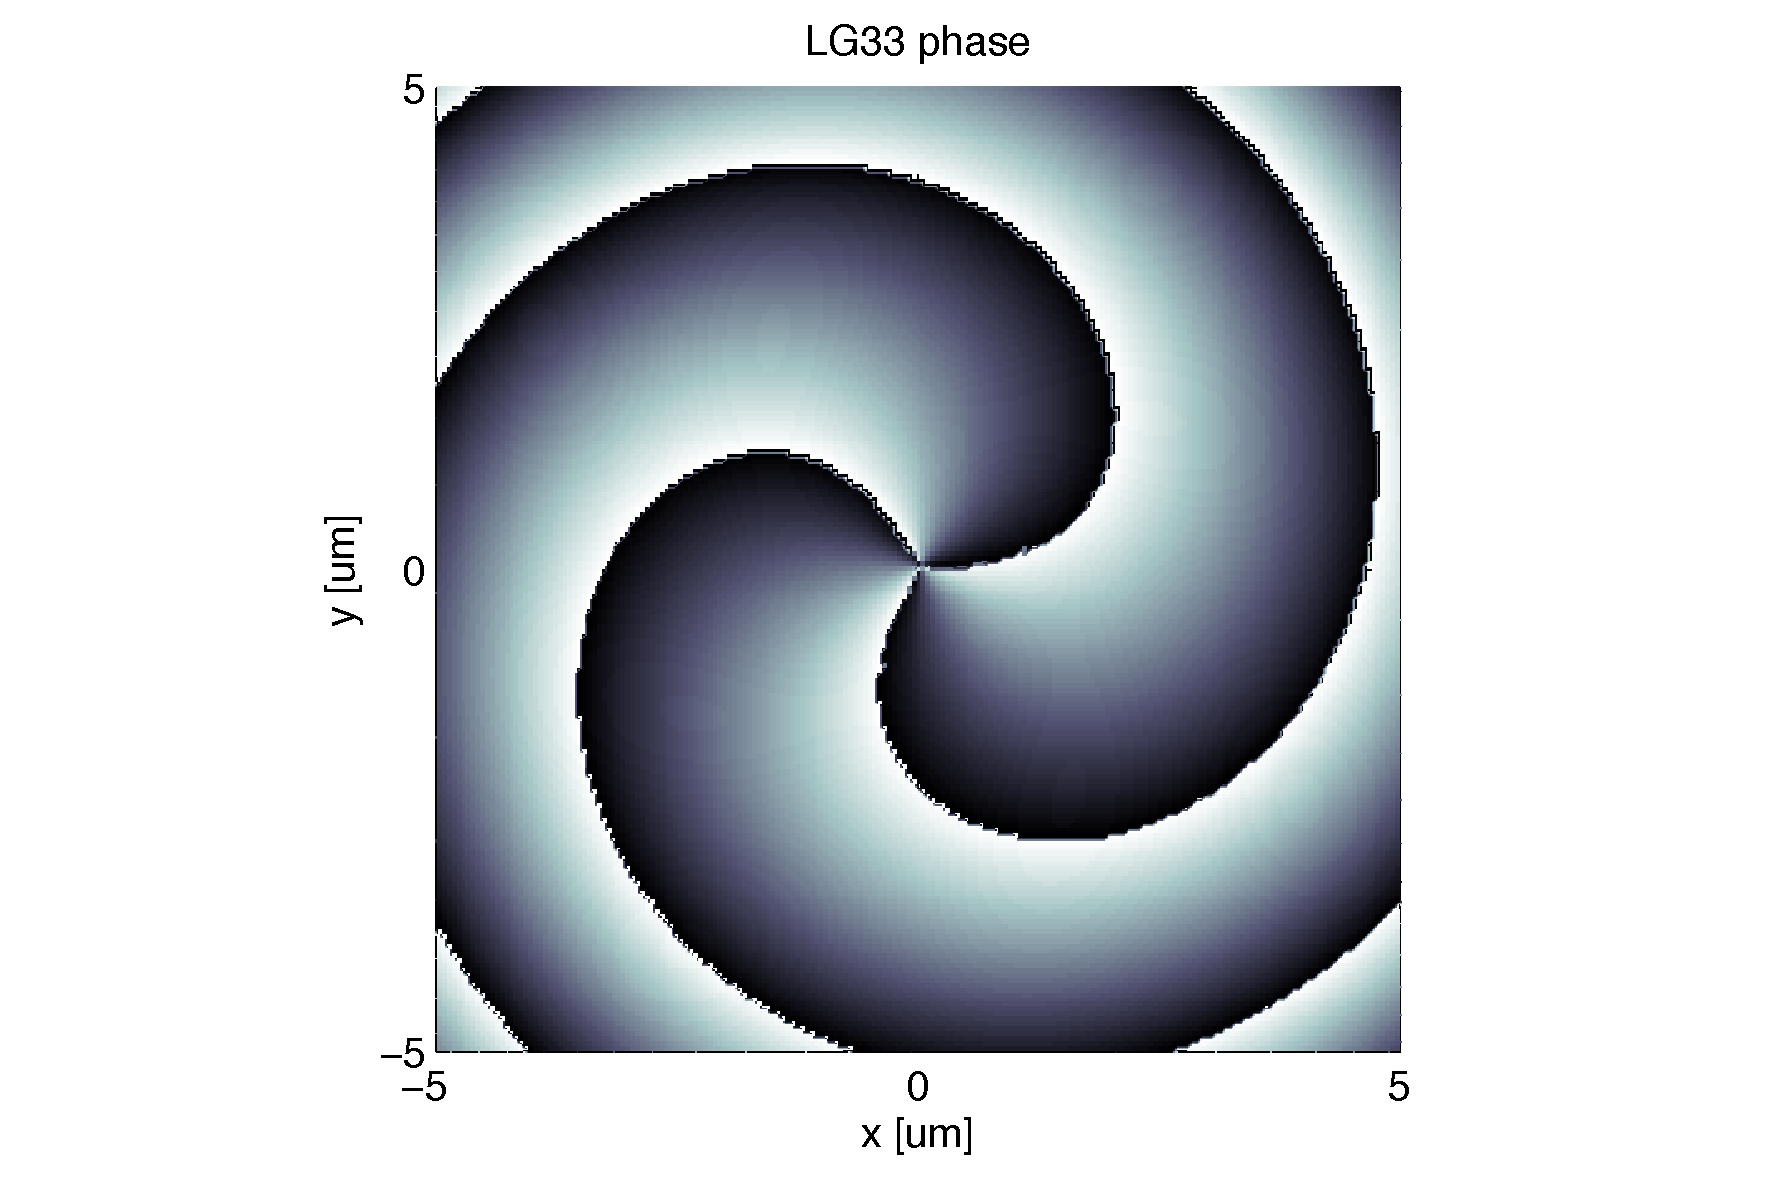
\includegraphics[width=0.47\textwidth, viewport=180 0 740 530]{Sec_Optics/LG33_phs}
\caption{The amplitude distribution of a LG$_{33}$ mode (left panel)
  shows a ring structure with 3 dark rings. The phase front of such a
  mode (right panel) is basically spherical with an additional helical
  structure superimposed.  
%That's why these modes are also called
%\emph{helical} Laguerre-Gauss modes. Mirrors with spherical surfaces
%can be used to build resonant cavities for such modes. 
}\label{Fig:LG33}
\end{figure}
%
The use of such a Laguerre-Gauss mode has been
selected for the ET design because it is directly compatible with 
other advanced technologies for the suppression of thermal or
quantum noise and does not requires a larger envelope or additional
interferometer hardware. Wherever possible optical design 
options have been analysed for the fundamental Gauss beam as
well as the LG$_{33}$ mode.
%
LG modes so far are
untested in high-precision interferometry.
%If the research and development process shows that this technique
%does not fulfil its promise, 
Several other alternatives are also under
active development, for example, Khalili cavities or wave guide
coatings, see~Appendix~\ref{Optics_App}.  These techniques can
be used as a drop-in replacement for LG modes without substantial
changes to the rest of the optical design.
}

\FloatBarrier
\subsubsection{A xylophone design for ET}\label{sec:xylophone}
\label{Xylophone}
Spanning the detection band over four orders of magnitude in frequency,
as is asked for third generation GW observatories such as ET,
is technically extremely challenging: different noise types dominate the various
frequency bands and often show opposite responses for different
tuning of the same design parameter.


In the following we give some examples of
fundamental issues of a broadband third generation interferometer that could be
resolved by using a set of xylophone detectors:
\begin{itemize}
\item \textbf{High Power vs Cryogenic Temperature}: Using a single broadband
ET observatory as described in \cite{HildETconventional} features the challenge of the
simultaneous use of high optical power (a few megawatts) to achieve the 
required high frequency sensitivity and test masses at cryogenic temperatures in 
order to provide the required suppression of thermal noise.
Even though tiny, the residual absorption of the
dielectric mirror coatings deposits heat in the mirrors which is difficult to extract,
without spoiling the performance of the seismic isolation systems. A possible
solution for this problem would be to build a xylophone observatory consisiting
of a high frequency detector featuring high power and high temperature and a
low frequency detector featuring low power and cryogenic temperatures.
\item \textbf{Shot Noise vs Radiation Pressure Noise}: Due to the fact that the shot 
noise contribution scales inverse with optical power, but the photon radiation
pressure noise contribution on the other hand  scales proportional to the optical power, it will be hard to obtain the desired bandwidth with a 
single detector. Therefore, again it might be useful
to split ET into a low-power low-frequency and a high-power high-frequency
companion.
\item \textbf{Mixing Interferometer Topologies}: Xylophone configurations would
also allow us to mix alternative interferometer topologies, such as Sagnac interferometer
\cite{Chen2003} and optical levers \cite{Khalili2002}, with the standard Michelson
 interferometer. For example one
could imagine that ET upgrades would feature a standard high-frequency Michelson interferometer
with a low-frequency optical lever as companion.
\end{itemize}

The xylophone concept was first suggested for Advanced LIGO,
 proposing to complement the standard broadband
 interferometers with an interferometer optimized for lower frequency,
 thus enhancing the detection of high-mass binary systems
\cite{Shoemaker2001LIGOXylophone, Conforto2004}.

One may think that a xylophone might significantly increase the required
hardware and its cost by the need to build more than one
 broadband instrument. However, such an argument
 does not take the technical
simplifications that it would allow, the better reliability of simpler instruments,
 and the more extensive scientific reach allowable into account.

For example splitting a third generation observatory into
a low-power, low-frequency  and a high-power high-frequency
interferometer, has not only the potential to resolve the above mentioned
conflict of photon shot noise  and photon radiation pressure noise, but
also allows to avoid the combination of high optical power and cryogenic test masses.
To reduce thermal noise to an acceptable level in the low frequency band, it is
expected that cryogenic suspensions and test masses are required.
Even though tiny, the residual absorption of the
dielectric mirror coatings deposits a significant amount of heat
 in the mirrors. Since this heat is difficult to extract,
without spoiling the performance of the seismic isolation systems, it imposes a
limit on the maximum circulating power of a cryogenic interferometer.

\begin{figure}[thbp]
\centering
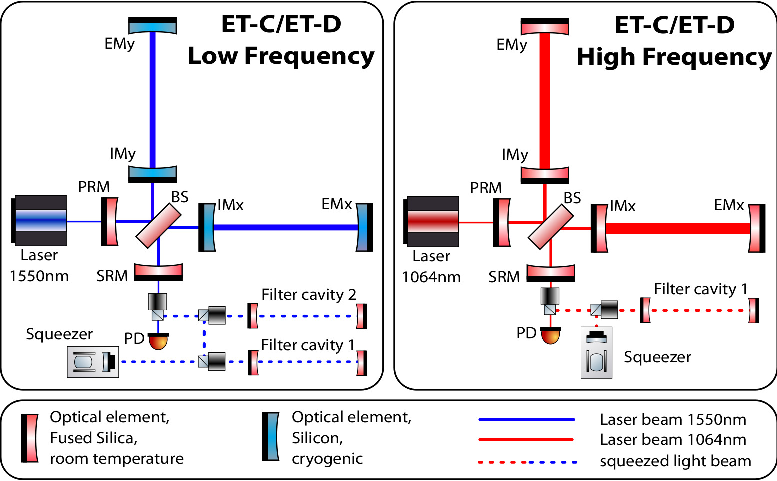
\includegraphics[width=0.8\textwidth]{Sec_Optics/Layout_overview.pdf}
\caption{Simplified sketch of the ET low and high frequency core interferometers of a single ET-detector.}
\label{Fig:opt_lay_over}
\end{figure}



\begin{table}
\begin{center}
\begin{tabular}{l l l}
\hline
\hline
Parameter & ET-D-HF   & ET-D-LF \\
\hline
Arm length & 10\,km & 10\,km \\
Input power (after IMC) & 500\,W & 3\,W \\
Arm power & 3\,MW & 18\,kW\\
Temperature & 290\,K &  10\,K  \\
Mirror material & fused silica & silicon \\
Mirror diameter / thickness & 62\,cm / 30\,cm & min 45\,cm/ T \\
Mirror masses & 200\,kg & 211\,kg \\
Laser wavelength & 1064\,nm & 1550\,nm \\
SR-phase & tuned (0.0) & detuned (0.6)\\
SR transmittance & 10\,\% & 20\,\% \\
Quantum noise suppression &  freq.\ dep.\ squeez.& freq.\ dep.\ squeez.\\
Filter cavities & $1 \times 10\,$km  & $2 \times 10\,$km\\
Squeezing level  & 10\,dB (effective) & 10\,dB (effective) \\
Beam shape &  LG$_{33}$& TEM$_{00}$\\
Beam radius & 7.25\,cm & 9\,cm \\
Scatter loss per surface & 37.5\,ppm & 37.5\,ppm \\
Seismic isolation & SA, 8\,m tall & mod SA, 17\,m tall \\
Seismic (for $f>1$\,Hz) & $5\cdot 10^{-10}\,{\rm m}/f^2$ & $5\cdot 10^{-10}\,{\rm m}/f^2$  \\
Gravity gradient subtraction & none & none \\
\hline
\hline
\end{tabular}
\caption{Summary of the most important parameters of the ET-D high and low frequency
interferometers. SA~=~super attenuator,  freq.\ dep.\ squeez.~=~squeezing
with frequency dependent angle.\label{tab:summary14}}
\end{center}
\end{table}

The baseline for ET is a 2-band xylophone detector configuration, composed of a
low-frequency (ET-LF) and a high-frequency (ET-HF) detector. Both interferometers
are Michelson interferometers featuring 10\,km armlength and an opening
angle of 60 degrees.  Due to their similar geometry both detectors will share
a single facility.
Table~\ref{tab:summary14} gives a brief overview of the main parameters
of the analysed low-frequency (ET-LF) and high-frequency (ET-HF) detector.
Figure~\ref{Fig:opt_lay_over}   shows sketches of the corresponding core
interferometers and the filter cavities. The full layout of the two core
interferometers of a single ET detector is depicted in Figure~\ref{Fig:Simple_ETv1}.


%\FloatBarrier
\subsubsection{Arm cavity design}
\label{sec:arm_cavity_design}

The size and shape of the laser beam inside the interferometer is
defined by the surface shape of the cavity mirrors; the beam sizes
at the arm cavity input mirrors (IM) and arm cavity end mirrors (EM) as well as the position of the cavity waist are determined
by only two parameters, the radii of curvature (ROC) of IM and EM.
Since inside the two Fabry-Perot cavities of the Michelson interferometer the
GW interacts with the laser light, creating signal sidebands, the two
arm cavities can be seen as the heart of the ET interferometers.
The characteristics of the arm cavities have not only a high impact
on the detector sensitivity and bandwidth, but also on the overall
detector performance.

The choice of the beam size on the arm cavity mirrors is a trade-off
process taking the following considerations into account:
\begin{itemize}
  \item For a given cavity length there is a minimal achievable beam size, which
is determined by the divergence of the beam.
\item Above this minimal beam size, any further increase in beam size leads to
and additional reduction of the various thermal noise contributions.
\item Finally the upper limit for the manageable beam size is given firstly by
the maximum available mirror substrate size and secondly by the approaching of
the cavity instability.
\end{itemize}

\longetbox{i}{hbox:beamwaist}{Beam waist of the arm cavity beam eigenmode}{
In the case of a two-mirror cavity the size of the beam can be
computed conveniently from the stability parameters $g_1$, $g_2$ defined
as:
\begin{equation}
	g_{1,2}=1-\frac{L}{R_{C\,1,2}}
\end{equation}
with $L$ the length of the cavity and $R_{C\,1,2}$ the radius of curvature
of the input and end mirror respectively.\\
%
The waist size $w_0$ of the cavity eigenmode can then be computed as :
\begin{equation}\label{eq:waist}
	w_0^2=\frac{L\lambda}{\pi}\sqrt{\frac{g_1g_2(1-g_1g_2)}{(g_1+g_2-2g_1g_2)^2}}
\end{equation}
%
In many cases a symmetric or near-symmetric cavity layout will be used (or can be used
to estimate design options). In that case we set
 $g=g_1=g_2$ which leads to a much simpler equation:
\begin{equation}\label{eq:waist_sym}
	w_0^2=\frac{L\lambda}{2\pi}\sqrt{\frac{1+g}{1-g}}=\frac{L\lambda}{2\pi}\sqrt{\frac{2R_{C}}{L}-1}
\end{equation}
%
%\textbf{Beam size on the arm cavity mirrors}
Typically we are interested in the size of the beam on the mirror, rather than
the waist size directly. The beam size can be computed similarly as the waists; for the input
mirror we get:
\begin{equation}\label{eq:spot}
	w_1^2=\frac{L\lambda}{\pi}\sqrt{\frac{g_2}{g_1(1-g_1g_2)}}
\end{equation}
And in the case of a symmetric cavity we obtain:
\begin{equation}\label{eq:spot_sym}
	w^2=\frac{L\lambda}{\pi}\sqrt{\frac{1}{1-g^2}}=\frac{\lambda}{\pi}\sqrt{\frac{R L}{2-\frac{L}{R}}}
\end{equation}
}

\textbf{Arm cavity mirror size}

A common method to define the mirror size is to demand the optical power loss
due to clipping (light being lost because it `falls over the edge of the
mirror') to be less than $1\,$ppm. The computation of the scaling factors is
described in~\cite{Chelkowski2009} and results in:
\begin{center}
\begin{tabular}{|l|c|c|}
	\hline
	mode  & TEM$_{00}$ & LG$_{33}$\\
	\hline
	mirror radius to beam  radius & 2.63 & 4.31\\
	\hline
\end{tabular}
\end{center}


\textbf{Minimal mirror sizes for ET}

Using the currently discussed options for ET we can compute minimal mirror sizes for various
options, by using $L=R_{C}$ resulting in $w_{\rm min}=\sqrt{\frac{L\lambda}{\pi}}$.
\begin{center}
\begin{tabular}{|l|c|c|}
	\hline
setup & min beam radius  & min mirror diameter \\
         & [cm] & [cm] \\
	\hline
LG$_{33}$, 1064\,nm  &  5.8      &  50.2     \\
	\hline
TEM$_{00}$, 1550\,nm  &  7.0      &   37.0    \\
	\hline
\end{tabular}
\end{center}




\textbf{Realistic mirror sizes for ET}

Using the minimal beam sizes is obviously not optimal in terms of
thermal noise. Therefore we intend to push the beam sizes for ET
towards the maximum feasible size, which corresponds to about 60\,cm
substrate diameter for fused silica mirrors and 50\,cm for the silicon mirrors.
Assuming 10\,km long arm cavities, we can derive the following arm cavity
characteristics.

\begin{center}
\begin{tabular}{|c|c|c|c|c|c|c|c|c|}
  \hline
IFO & $\lambda$& beam shape & mirror diameter & $R_{\rm C}$ & $w_0$ &$z_0$ & $w$ & $z_{\rm R}$ \\
\hline
ET-HF & 1064\,nm & LG$_{33}$ & 62\,cm & 5691\,m & 2.51\,cm & 5000\,m & 7.2\,cm & 1859\,m\\
\hline
ET-LF & 1550\,nm & TEM$_{00}$ & 45\,cm &5577\,m & 2.9\,cm & 5000\,m & 9.0\,cm & 1698\,m\\
\hline
\end{tabular}
\end{center}

%and the corresponding effects of parametric instabilities are analysed in section~\ref{sec:opt_layout_PI}.

%\FloatBarrier
%\subsubsection{Parametric instability}
%\emph{
%Author: \textbf{Kazuhiro Yamamoto, Daniel Heinert, Sergey E. Strigin}\\
%}
%\label{sec:opt_layout_PI}
%
%Parametric instability is one of the important issues in future
%interferometric detectors \cite{Braginsky2001}. Such interferometers
%have at least a few km length arm cavities. The spectral distance between 
%optical modes in these long cavities are on the order of 10 kHz.
%This value is comparable with the frequencies of elastic modes of
%the cavity mirrors. In such cases, the parametric instability
%becomes a serious problem in the stable operation of
%interferometers. A small thermally driven elastic vibration
%modulates the light and excites the transverse optical modes of the
%cavity which is called Stokes modes. These excited optical modes apply modulated radiation
%pressure on the mirrors. This makes the amplitude of the elastic
%modes larger. At last, the elastic modes and optical Stokes modes which is 
%different from injected beam oscillate largely. This is the parametric instability.
%
%The formula of the parametric instability of a Fabry-Perot cavity
%(without anti-Stokes modes) is derived in Ref. \cite{Braginsky2001}.
%If the parametric gain $R$ of an elastic mode is larger than unity, that
%mode is unstable. The formula of $R$ is
%\begin{equation}
%R = \sum_{\rm optical\ mode} \frac{4PQ_{\rm m}Q_{\rm
%o}}{McL{\omega_{\rm m}}^2} \frac{\Lambda_{\rm o}}{1+\Delta
%\omega^2/{\delta_{\rm o}}^2}, \label{R}
%\end{equation}
%where $P,Q_{\rm m},Q_{\rm o},M,c,L,\omega_{\rm m},\Delta\omega$,
%and $\delta_{\rm o}$ are the optical power in the cavity, the
%Q-values of the elastic and optical modes, the mass of the mirror,
%the speed of light, the cavity length, the angular frequency of
%the elastic mode, the angular frequency difference between the
%elastic and optical modes, and the half-width angular frequency of
%the optical mode, respectively. The value $\Lambda_{\rm o}$
%represents the spatial overlap between the optical and elastic
%modes. If the shapes of the optical and elastic modes are similar,
%$\Lambda_{\rm o}$ is on the order of unity. If the shapes are not
%similar, $\Lambda_{\rm o}$ is almost zero. When the shapes and
%frequencies of the optical and elastic modes are similar
%($\Lambda_{\rm o} \sim 1, \Delta \omega \sim 0$), $R$ will become
%several thousands in second generation projects; Advanced LIGO and 
%Advanced Virgo. In these projects, the effect of parametric
%instability is a serious problem \cite{Ju2006a,Ju2006b}. 
%
%Here, the parametric instability of the Einstein Telescope
%(ET) interferometer is discussed. This instability depends on the
%specification of the interferometer. However, details of
%the design are considered and discussed now. Therefore, outlines of
%the instability of the ET interferometer, preliminary calculation results, 
%and future work are shown. In
%order to simplify the discussion, only the instability of a
%Fabry-Perot cavity is considered. The effect of power and signal
%recycling (or resonant sideband extraction) techniques are not taken into
%account.
%
%At first, we consider the parametric instabilities in Advanced LIGO
%as an example of the second generation.
%%In order to calculate $\omega_{\rm
%%m}$ and $\Lambda_{\rm o}$ for the instability evaluation, we used
%%ANSYS, which is a software application for a finite-element
%%method.
%At second, the parametric instability in ET is
%discussed (outline of instability in ET and the preliminary results of calculation 
%are shown). At third, how to suppress the instability of the ET
%arm cavity is considered. The last part is devoted to a
%summary (and future work).
%
%\textbf{Parametric instability of the second generation interferometers}
%\nopagebreak
%
%As example of the second generation interferometers, the Advanced LIGO is considered. The specifications of 
%Advanced Virgo are similar. Table \ref{tab:specification2} gives the specifications of Advanced
%LIGO in Refs. \cite{Ju2006a,Ju2006b,Zhao2005} (after these references, the
%specifications of Advanced LIGO were changed). 
%  
%Study of the instability in Advanced LIGO by a group at the
%University of Western Australia \cite{Ju2006a,Ju2006b} is reviewed
%briefly. They investigated what happens when the curvature of a
%mirror is changed. The curvature of the other mirror is the
%default value given in Table \ref{tab:specification2}. Reference
%\cite{Ju2006b} shows the curvature dependence of the unstable mode
%number. 
%The number of the unstable modes of mirror cavity is between 20 and 60 
%(it must be noted that this number increases if the higher elastic modes are taken into account). 
%Reference \cite{Ju2006a} shows that the
%maximum of $R$ in the various elastic modes strongly depends on
%the mirror curvature. Even a shift of only a few meters in the
%mirror curvature causes a drastic change of the maximum $R$. The
%requirement of the accuracy in the mirror curvature in Advanced
%LIGO is difficult to be achieved.
%
%\textbf{Parametric instability of Einstein Telescope: Specifications of Einstein Telescope}
%\nopagebreak
%
%Here, the parametric instability of the ET is
%considered. The details of the ET interferometer are not decided
%now. Here, we adopt parameters of ET-C \cite{Hild2010a}. 
%These parameters are summarized in Table
%\ref{tab:specification2}. Parameters of ET-D \cite{Hild2010b} (this is newer than ET-C) 
%are similar to those of ET-C. 
%The difference does not change the paremetric instability. The comparison with old sensitivity,
%ET-B \cite{HildETconventional,Yamamoto2009}, is also discussed here.  
%\begin{table}[h]
%\begin{center}
%\begin{tabular}{llll}
%\hline
%\hline
% &Advanced LIGO&ET-C-HF&ET-C-LF\\
%\hline
%Laser beam profile&Gaussian&LG33&Gaussian\\
%Wavelength($\lambda$)&1064 nm&1064 nm&1550 nm\\
%Cavity length($L$)&4000 m&10000 m&10000 m\\
%Front mirror curvature radius($R_1$)&2076 m&5643 m&6109 m\\
%End mirror curvature radius($R_2$)&2076 m&5643 m&6109 m\\
%Beam radius at the mirrors($w_{\rm i}$)&60 mm&72.5 mm&120 mm\\
%Finesse (${\cal F}$) & 1250 & 850 & 850 \\
%Power in a cavity($P$) &0.83 MW&3 MW&18 kW\\
%Mirror material&Fused silica&Fused silica&Silicon\\
%Sound velocity in mirror ($v$) &5.7 km/s&5.7 km/s&8.4 km/s\\
%Density of mirror ($\rho$) &2.2 g/cm$^3$&2.2 g/cm$^3$&2.3 g/cm$^3$\\
%Mirror mass($M$)&40 kg&200 kg& 211 kg \\
%Mirror diameter($r$)&340 mm&620 mm&620 mm\\
%Mirror thickness($t$)&200 mm&300 mm&300 mm\\
%Mirror temperature($T$)&300 K&300 K&10 K\\
%\hline
%\hline
%\end{tabular}
%\end{center}
%\caption{Specification of Advanced LIGO
%\cite{Ju2006a,Ju2006b,Zhao2005}, and ET-C
%\cite{Hild2010a}.\label{tab:specification2}}
%\end{table}
%
%%Hild did not show the curvatures of mirrors. The curvature in Table
%%\ref{tab:specification2} was derived from his parameters, cavity
%%length and beam radii at mirrors. It is supposed that the
%%curvature of front and end mirrors is the same. The beam radius
%%$w_{\rm i}$ at mirror is described as
%%\begin{eqnarray}
%%{w_{\rm i}}^2 &=& \frac{L \lambda}{\pi |g_{\rm i}|}\sqrt{\frac{g_1 g_2}{1- g_1 g_2}}, \\
%%g_{\rm i} &=& 1- \frac{L}{R_{\rm i}}.
%%\end{eqnarray}
%%Since $w_{\rm i}$ is 12 cm and $L$ is 10 km, the curvature of the
%%mirrors is 5070 m.
%
%%Hild supposed that the mass of a mirror $M$ is 120 kg. It implies
%%that the aspect ratio (the ratio of the mirror thickness to
%%diameter) is smaller than those of usual interferometric
%%gravitational wave detectors because of the large beam radius (12
%%cm). However, in order to simplify the discussion, it is assumed
%%that the aspect ratio is the same as usual one (0.6 in LCGT). The
%%mirror radius must be at least 2.5 times larger than the beam
%%radius because the diffraction loss must be enough small
%%\footnote{In this case, the diffraction loss is 3.7 ppm.}. Thus,
%%the mirror radius of ET is 30 cm. The mirror radius of LCGT is
%%12.5 cm. The volume of a mirror of ET is $(30/12.5)^3=2.4^3=14$
%%times larger than that of LCGT. The mirror mass of LCGT is about
%%30 kg. If the ET mirrors are made from sapphire as like LCGT, the
%%mirror mass of ET is 410 kg. If the ET mirrors are made from
%%silicon (densities of silicon and sapphire are 2.3 g/cm$^3$ and 4
%%g/cm$^3$), the mirror mass is 230 kg.
%
%\textbf{Parametric instability of Einstein Telescope: Maximum of R of Einstein Telescope}
%\nopagebreak
%
%The strength of instability $R$ is written as
%\begin{equation}
%R \propto \frac{4PQ_{\rm m}Q_{\rm o}}{McL{\omega_{\rm m}}^2}.\label{Rmax}
%\end{equation}
%Let us compare the maximum $R$ of ET
%with that of Advanced LIGO. It is supposed that $Q_{\rm m}$ is the same. 
%We must take the difference of power $P$ and mass $M$ into account. 
%It must be noted that the ratio $Q_{\rm o}/L$ is proportional to the factor ${\cal F}/\lambda$.
%The resonant frequency 
%$\omega_{\rm m}$ is inversely propotional to the mirror size. 
%It is assumed that scale of mirror is propotional to the third root of 
%mirror volume (ratio of mass to density). 
%We should consider the material difference in the case of ET-LF. 
%The resonant frequency of mirror $\omega_{\rm m}$ is inversely propotional to the sound velocity.
%
%The ratio of $R$ of ET-HF to that of Advanced LIGO is 
%\begin{equation}
%\left(\frac{3 {\rm MW}}{0.83 {\rm MW}}\right)\left(\frac{850}{1250}\right) \left(\frac{40 {\rm kg}}{200 {\rm kg}}\right) \left(\frac{200 {\rm kg}}{40 {\rm kg}}\right)^{2/3}=1.4.
%\end{equation}
%The ratio of $R$ of ET-LF to that of Advanced LIGO is 
%\begin{equation}
%\left(\frac{18 {\rm kW}}{0.83 {\rm MW}}\right)\left(\frac{850}{1250}\frac{1064~{\rm nm}}{1550~{\rm nm}}\right) \left(\frac{40 {\rm kg}}{211 {\rm kg}}\right) \left(\frac{211 {\rm kg}}{40 {\rm kg}}\frac{2.2 {\rm g/cm}^2}{2.3 {\rm g/cm}^3}\right)^{2/3} \left(\frac{5.7 {\rm km/s}}{8.4 {\rm km/s}}\right)^2=2.6\times10^{-3}. 
%\end{equation}
%The maximum of $R$ in Advanced LIGO is on the order of 100 \cite{Ju2006b}. Therefore, the parametric instability of ET-LF 
%is not a problem. On the other hand, maximum $R$ of ET-HF is comparable with that of Advanced LIGO. We will discuss 
%parametric instability of only ET-HF.
%
%\textbf{Parametric instability of Einstein Telescope: Number of unstable modes of ET-C-HF}
%\nopagebreak
%
%The number of unstable modes are proportional to the product of elastic mode density and 
%optical mode density.
%The mode density of the elastic mode is proportional to the cubic
%of the ratio of the mirror size to the sound velocity. Thus, 
%the elastic mode density of ET-HF is 5 times larger than that of Advanced LIGO because
%of the difference of mirror size. 
%
%The ratio of the optical transverse mode interval to the free spectrum range is
%described as
%\begin{eqnarray}
%&&\frac1{\pi}\cos^{-1}\sqrt{g_1 g_2},\\
%&&g_n = 1-\frac{L}{R_n}.
%\end{eqnarray}
%There are 8 and 4 transverse optical modes in a free spectrum
%range of Advanced LIGO and ET-HF interferometers. Since the cavity of ET is 2.5
%times longer, the free spectrum range is 2.5 times smaller.
%Therefore, the optical mode density of the ET-HF interferometer is 1.4 times larger.
%The reason why the optical mode density of ET-HF is comparable with that of Advanced LIGO 
%nevertheless the cavity length of ET-HF is longer stems from the difference of beam shape, 
%TEM$_{00}$ and LG$_{33}$. Since the beam in Advanced LIGO is Gaussian (TEM$_{00}$), a larger beam radius 
%implies smaller interval between optical transverse modes. On the other hand, ET-HF adopts 
%the LG33 mode, higher optical transverse mode. The radius of higher mode is larger than that of TEM00. 
%Thus, it is not necessary to increase the radius of fundamental mode (TEM$_{00}$). This effect cancels 
%that of longer length of cavity. 
% 
%In total, the number of the instable modes, which is proportional
%to the product of the elastic and optical mode densities, of the
%ET-HF interferometer is 7 times larger than that of the Advanced LIGO interferometer. 
%The main reason of the difference of Advanced LIGO and ET-HF is that of size of mirrors. 
%
%\textbf{Parametric instability of Einstein Telescope: Mirror curvature dependence of ET-C-HF}
%\nopagebreak
%
%The instability strength $R$ is a function of the transverse optical
%mode frequencies. How the curvature variation affects
%the $n$-th optical transverse mode was calculated.
%The result is 1.2$n$ Hz/m in ET-HF. This value is smaller than that of 
%Advanced LIGO (15$n$ Hz/m). The longer baseline and adopting LG33 mode 
%make mirror curvature dependence of instability smaller. 
%
%\textbf{Parametric instability of Einstein Telescope: Comparison with ET-B}
%\nopagebreak
%
%Here parametric instability of ET-B \cite{HildETconventional}, which is sensitivity in old design, 
%is compared with that of ET-C (the details about parametric instability of ET-B is 
%discussed in Ref.~\cite{Yamamoto2009}). 
%From point of view of parametric instability, ET-C is better than ET-B.
%Obviously, the first reason is that ET-C-LF has no serious problem about this instability. 
%The second reason is that ET-C-HF has (about 4 times) less instable modes and (about 3 times) 
%weaker mirror curvature dependence.
%This is because of the difference of beam shape; Gaussian beam (TEM00) in ET-B and LG33 in ET-C-HF. 
%
%\textbf{Parametric instability of Einstein Telescope: Preliminary results of calculation for parametric instability of ET-C-HF using finite element method}
%\nopagebreak
%
%%{\bf The details will appear here.}
%
%%{\bf I hope that the details of ET-C-HF can be discussed. Daniel Heinert and Sergey Strigin will calculate it.}
%
%%{\bf 
%The preliminary calculation for instability of ET-C-HF using finite element method 
%is introduced here. At first, it must be noted that 
%further investigation is necessary.
%We consider all elastic modes below 30~kHz (twice times the free spectral range of cavity). The anti-Stokes modes are 
%taken into account. Therefore, Eq.~(\ref{R}) should be rewritten as \cite{Kells2002}
%\begin{equation}
%R = \sum_{\rm optical\ mode} \frac{4PQ_{\rm m}Q_{\rm
%o}}{McL{\omega_{\rm m}}^2} \frac{\Lambda_{\rm o}}{1+\Delta
%\omega^2/{\delta_{\rm o}}^2}-\sum_{\rm optical\ mode(anti)} \frac{4PQ_{\rm m}Q_{\rm
%{o(anti)}}}{McL{\omega_{\rm m}}^2} \frac{\Lambda_{\rm o(anti)}}{1+\Delta
%\omega_{\rm anti}^2/{\delta_{\rm o(anti)}}^2}, \label{R_antiStokes}
%\end{equation}
%The number of unstable modes is only 5. One of the reasons is that some Stokes modes are canceled by 
%anti-Stokes modes effectively. If the anti-Stokes modes are neglected, there are 17 unstable modes. 
%In this calculation, the splitting of the degenerated elastic mode due to imperfectness of mirrors 
%is not taken into account \cite{Strigin2008a,Strigin2008b}. 
%Since this effect increases the number of unstable modes, it should be considered in a next step. 
%%However, even if the anti-Stokes modes are neglected, the number of unstable modes is smaller than 
%%Advanced LIGO (20$\sim$60). Previous discussion predicts that number of unstable modes is about 7 times 
%%larger than that of Advenced LIGO. The reason should be investigated. One of the possible reasons is that 
%%beam shape (LG33) is not taken into account in previous discussion, i.e.\ the complicate beam shape might 
%%make $\Lambda_{\rm o}$ smaller (Daniel and Sergey are comparing the overlap factors for some modes of the
%%ET-HF standard configuration. Some results?). 
%
%We calculated the instability with the other mirror curvature. 
%The curvature of one mirror is changed. The new curvature is 5743~m.
%In this case, the number of unstable modes is 5. 
%So, the number of unstable modes does not depend on mirror curvature 
%supporting the conclusion of the previous discussion.
%
%%Shape of optical and elastic modes in the worst case (highest $R$)?}
%
%\textbf{Instability suppression in ET-C-HF}
%\nopagebreak
%
%Although the strength of the instability of the ET-HF interferometer
%is comparable with that of Advanced LIGO, the number of
%the unstable modes is 7 times larger. The three methods for the
%instability suppression in Advanced LIGO are being studied
%\cite{Ju2006b,Gras2006,Ju2009}. Let us consider whether these three
%methods (thermal tuning method, feedback control, Q reduction of
%elastic modes) are appropriate for ET (the tranquilizer cavity
%\cite{Braginsky2002} is one of the other methods. However, this
%is not introduced here).
%
%%{\bf I think something should be added.}
%
%\textbf{Instability suppression in ET-C-HF: Thermal tuning method}
%\nopagebreak
%
%In the thermal tuning method \cite{Ju2006b}, a part of the mirror is
%heated for curvature control. Since $R$ depends on the curvature,
%the suppression of $R$ should be possible by this manner. However,
%this method is not useful in ET-HF because the mirror curvature dependence of 
%parametric instability is 10 times smaller than that of Advanced LIGO. 
%
%\textbf{Instability suppression in ET-C-HF: Feedback control}
%
%It is possible to control the light or the mirror so that the
%parametric instabilities would be actively suppressed \cite{Ju2006b,Ju2009}.
%If the number of unstable modes is smaller, feedback control is
%easier. However, these are more difficult (active) methods than Q
%reduction (passive method) of the elastic modes, especially, if
%there are many unstable modes. Therefore, it is good that 
%almost all modes are suppressed by passive method and that 
%only strong instable modes are supressed by active method. 
%
%\textbf{Instability suppression in ET-C-HF: Q reduction of elastic modes}
%\nopagebreak
%
%%\begin{figure}[thbp]
%%\centering
%%\includegraphics[width=0.8\textwidth]{Sec_Optics/coatingPI.pdf}
%%\caption{Loss on the barrel surface. Although this loss decreases the
%%elastic Q-values of the mirror, $Q_{\rm m}$, it has only a small
%%contribution to the thermal noise \cite{Levin1998,Yamamoto2006}. Thus,
%%this loss suppresses the parametric instabilities without an
%%increase of the thermal noise \cite{Gras2006,Gras2004}.}
%%\label{Fig:opt_coatingPI}   
%%\end{figure}
%
%
%This is a useful method \cite{Gras2006} for ET. The value of
%$R$ is proportional to the Q-value of the elastic mode, $Q_{\rm
%m}$, as shown in Eq. (\ref{R}). The Q-values of fused silica 
%are about $10^8$ \cite{Numata2004}. The
%maximum $R$ of ET is comparable with that of Advanced LIGO, on the order of 100
%hundreds at most \cite{Ju2006b}. If the Q-values of the ET-HF mirrors become $10^6$, 
%almost all modes become stable. Since
%the mechanical loss concentrated far from the beam spot has a
%small contribution to the thermal noise \cite{Levin1998,Yamamoto2002},
%we should be able to apply additional loss on a barrel surface 
%%as in Fig. \ref{coatingPI}, 
%%without sacrificing the thermal noise
%\cite{Gras2006,Gras2004}. 
%The thermal noise caused by loss on barrel surface is 
%$4.3 \times 10^{-25}/\sqrt{\rm Hz}$ at 100~Hz (details are described 
%in Appendix after the summary of parametric instability). This is comparable with ET-HF sensitivity. 
%However, this estimation is not precious (in order to simplify the discussion, 
%it is assumed that laser beam is Gaussian although it is LG33). We should investigate thermal noise 
%introduced by loss on barrel surface. 
%%I hope that Daniel Heinert and Sergey Strigin will provide useful supports.}
%
%We are able to introduce the loss on the barrel surface by the
%coating Ta$_2$O$_5$, which is a popular material for the
%reflective coating of the mirrors. According to Ref.
%\cite{Yamamoto2006}, the loss angle of the
%SiO$_2$/Ta$_2$O$_5$ coating is $(4 \sim 6) \times 10^{-4}$ between
%4 K and 300 K. Since the loss of this coating is dominated by that
%of Ta$_2$O$_5$ \cite{Penn2003}, the loss angle of Ta$_2$O$_5$ is $(8
%\sim 12) \times 10^{-4}$. If the barrel loss dominates the mirror
%Q, it would be expressed as \cite{Yamamoto2002}
%\begin{equation}
%\frac1{Q_{\rm m}} \sim \frac{E_{{\rm Ta}_2{\rm O}_5}}{E_{\rm substrate}}
%\frac{2 d}{R}\phi,
%\label{1/Qm}
%\end{equation}
%where $E_{{\rm Ta}_2{\rm O}_5},E_{\rm substrate}, d, R, \phi$ are
%the Young's moduli of Ta$_2$O$_5$ and the mirror substrate, the
%thickness of the Ta$_2$O$_5$ layer, the mirror radius and the loss
%angle of Ta$_2$O$_5$, respectively. These values are summarized in
%Table \ref{tab:coatingspe} \cite{Hild2010a, Yamamoto2006}. In order
%to arrive at Q-values of $Q_{\rm m} \sim 10^6$, the Ta$_2$O$_5$ coating
%thickness $d$ must be 80 $\mu$m in the case of ET-HF. 
%\begin{table}[h]
%\begin{center}
%%\begin{ruledtabular}
%\begin{tabular}{ll}
%\hline
%\hline
%Young's modulus of the Ta$_2$O$_5$ ($E_{{\rm Ta}_2{\rm O}_5}$)
%&$1.4 \times 10^{11}$ Pa\\
%Young's modulus of the fused silica &$7.2 \times 10^{10}$ Pa\\
%Mirror radius ($R$)&31 cm\\
%Loss angle of Ta$_2$O$_5$ ($\phi$)&$10^{-3}$\\
%\hline
%\hline
%\end{tabular}
%%\end{ruledtabular}
%\end{center}
%\caption{Specification of the coating
%\cite{Hild2010a, Yamamoto2006}.\label{tab:coatingspe}}
%\end{table}
%
%Recently, another method to reduce Q-values of elastic mode (using electrostatic actuator) is proposed 
%\cite{Miller2011}. 
%It should be considered in near future. 
%
%\etbox{i}{box:result}{Summary}
%{The parametric instability of ET-C is discussed 
%(it is expected that the result of ET-D is similar). 
%%It is better than that of ET-B. 
%The instability of ET-C-LF is not a serious issue because of the small light power. 
%The maximum strength of instability of ET-C-HF is comparable to that of Advanced LIGO. 
%The mirror curvature depepndence of ET-C-HF instability is about 10 times 
%weaker than that of Advanced LIGO because of longer baseline and LG33 beam.
%However, the instable mode number is 7 times larger (In order to evaluate a precise number, 
%the calculation using finite element method is necessary. This calculation is in progress). 
%This is mainly owing to the larger mirrors of ET.
%We should investigate how to suppress. 
%Feedback control and Q reduction of elastic modes are candidates.}
%
%\textbf{Appendix A : Mirror scale dependence of thermal noise by barrel surface loss}
%\nopagebreak
%
%The ET mirror is larger than the Advanced LIGO mirror. We must consider the
%size effect on the thermal noise by the loss on the barrel surface. In order to
%simplify the discussion, it is supposed that the mirror and laser
%beam of ET are similar to those of Advanced LIGO (although the beam of ET-HF is 
%LG33, not Gaussian). In short, the difference
%between ET and Advanced LIGO mirrors is only the scale. The ratio of beam
%radius to mirror radius is the same.
%%In order to simplify the discussion,
%%it is supposed that the beam radius and thickness of loss layer on
%%barrel surface is proportional to mirror radius and that the ratio
%%of mirror thickness to mirror diameter is constant.
%Under these assumptions, Q-values of mirrors are independent of the
%mirror scale, $a$. According to Ref. \cite{Levin1998}, the amplitude
%of the thermal noise $\sqrt{G_{\rm coating}}$ is described as
%\begin{equation}
%\sqrt{G_{\rm coating}} \propto \sqrt{W_{\rm diss}},
%\label{Levin}
%\end{equation}
%where $W_{\rm diss}$ is the dissipated power when the pressure of
%which the profile $p(r)$ is the same as the laser beam is applied
%on the mirror flat surface. If the loss is the structure damping,
%the dissipated power is proportional to the elastic energy in the
%loss layer on the barrel surface;
%\begin{equation}
%W_{\rm diss} \propto \int_{\rm barrel\ surface} {\cal E} dS \times d,
%\label{Wdiss}
%\end{equation}
%where ${\cal E}$ and $d$ are the elastic energy density and the thickness of
%the loss layer. The problem is how $W_{\rm
%diss}$ depends on the mirror scale $a$. Since the mirrors are
%similar, $dS$ and $d$ are described as
%\begin{eqnarray}
%dS &\propto& a^2,\\
%d &\propto& a.
%\end{eqnarray}
%The elastic energy density ${\cal E}$ is proportional to the
%square of the strain tensor. The strain tensor is proportional to
%the pressure on the flat surface $p$. This pressure is inverse
%proportional to the square of the scale. In short, the elastic
%energy density is written as
%\begin{equation}
%{\cal E} \propto p^2 \propto \frac1{a^4}.
%\end{equation}
%We are able to obtain the relationship between the thermal noise
%and the mirror scale;
%\begin{equation}
%\sqrt{G_{\rm coating}} \propto \sqrt{\frac1{a^4} \times a^2 \times a} = \sqrt{\frac1{a}}.
%\label{parametric instability size correction}
%\end{equation}
%
%Above discussion is based on the assumption that the ratio of the
%beam radius to mirror radius is constant. If the mirror size is
%fixed, the thermal noise by the barrel loss is independent of the beam size
%\cite{Yamamoto2002}. Therefore, the thermal noise by the barrel
%surface coating is inverse proportional to the square root of the
%mirror scale.
%
%The thermal noise caused by surface coating for instability supression is evaluated. The 
%thermal noise by the holes with loss on the barrel surface is investigated in Ref. \cite{Gras2004}.
%The size of their mirror is 150~mm in diameter and 60~mm in thickness. The mass is 2.3~kg. Since 
%the mass of ET-HF is 200~kg, the size of ET-HF mirror is about $(200/2.33)^{1/3}\sim4.4$ times larger.
%The beam radius of ET-HF is 72.5~mm. If the ratio of beam radius to mirror radius is the same, 
%the beam radius of ET-HF corresponds to 1.6~cm in Ref. \cite{Gras2004}. Figure 4 of Ref. \cite{Gras2004} 
%shows that mirror thermal noise (displacement) with 1.6~cm radius beam is about $10^{-20}~{\rm m/}\sqrt{\rm Hz}$ at 100~Hz. 
%Since there are 4 mirrors and cavity length is 10~km, it corresponds to 
%a strain noise amplitude of $2 \times 10^{-24}~/\sqrt{\rm Hz}$.
%We should take correction of size, Eq.~(\ref{parametric instability size correction}), into account.  
%The Q-values of mirror with this loss in Ref.~\cite{Gras2004} 
%is $1/(10^{-2}\times5\times10^{-4})=2\times10^5$. Since we assume 
%that Q-value is $10^{6}$, we should take this difference into account. In total,
%\begin{equation}
%2 \times 10^{-24}~/\sqrt{\rm Hz} \times \sqrt{\frac{1}{4.4}} \times \sqrt{\frac{2 \times 10^5}{10^6}} = 4.3 \times 10^{-25}~\sqrt{\rm Hz}
%\end{equation}
%This value is comparable with the ET-HF sensitivity. 
%However, this evaluation is not precise. For example, we assumed that beam is Gaussian. 
%However, ET-HF will adopt LG beam. These effects should be investigated. 
%%I hope that Daniel Heinert and Sergey Strigin will provide useful supports.}

\FloatBarrier
\subsubsection{Central interferometer design}
\label{sec:opt_layout_CITF}

The central interferometer consists of the two recycling cavities and the
central Michelson interferometer formed by the beam splitter and the arm cavity
input mirrors.
The design of the central interferometer is mainly determined by two
constraints. First of all it should allow for the implementation of
non-degenerate recycling cavities. Second, the central interferometer has to
serve as mode-matching telescope for the arm cavities.

The non-degenerate recycling cavity design used by the advanced detectors
(see Figure~\ref{Fig:Sec_Optics_AdvLIGO_IFO_Schematic}) can probably not be
directly adapted for ET, because no beam splitter substrates of the required dimensions
would be available. For example the high frequency interferometer featuring an opening
angle of  60 degree would require a beam splitter with a diameter of 115\,cm.

Therefore we plan to investigate design options making use of input
mirror substrates including a focussing lens with a focal length of 0.2 to 1\,km
and shifting the input mirrors away from the beam splitter.  Figure~\ref{Fig:Simple_ETv1}
illustrates how such a configuration would look like. Please note that the arm cavity mirrors are the only full sized optical
elements and that beam splitter and recycling mirrors can be significantly smaller. In addition in this scenario no
additional folding mirrors are necessary in the recycling cavities.

\textbf{Layout option for TEM$_{00}$, 1550\,nm}
\nopagebreak

The optical parameters
of a possible solution based on a arm cavity length of
$L=10$\,km and a TEM$_{00}$ mode at 1550\,nm are provided below:
\begin{itemize}
\item focussing element in or near the ITM with a focal length of $f=303$\,m
\item distance ITM--BS: 300\,m
\item distance BS--MPR: 10\,m
\item beam size on BS: 6\,mm
\item beam size on MPR: 3.4\,mm
%\item Rayleigh range in central interferometer: 6.3\,m
\end{itemize}

The recycling cavity formed by MPR and ITM has a length of
310\,m and a free spectral range of 484\,kHz. The round-trip Gouy phase
is given by $\approx 9.6$\,deg which
corresponds to a mode separation frequency of $25.8$\,kHz.

\textbf{Layout option for LG$_{33}$, 1064\,nm}
\nopagebreak

Using the same distances and focussing elements for the interferometer
with a LG$_{33}$, 1064\,nm beam, we also obtain reasonable numbers:
\begin{itemize}
\item beam size on BS: 4.7\,mm
\item beam size on MPR: 2.7\,mm
%\item Rayleigh range in central interferometer: 6.7\,m
\item Gouy phase: 10.5\,deg
\item mode separation frequency:  28.1\,kHz
\end{itemize}

These layout options are not yet optimised but they show that a
separation between beam splitter and input optics in the order of 300\,m
represents a useful baseline. The numbers for the beam sizes at the
beam splitter and recycling mirrors in both cases need to be checked against a
detailed thermal noise computation.

Furthermore, the design needs to be evaluated for losses originating
from astigmatisms inside the recycling cavities as well as for scattered
noise issues.


%Deduced requirements (link to Sec.~\ref{sec:optcomps}) 